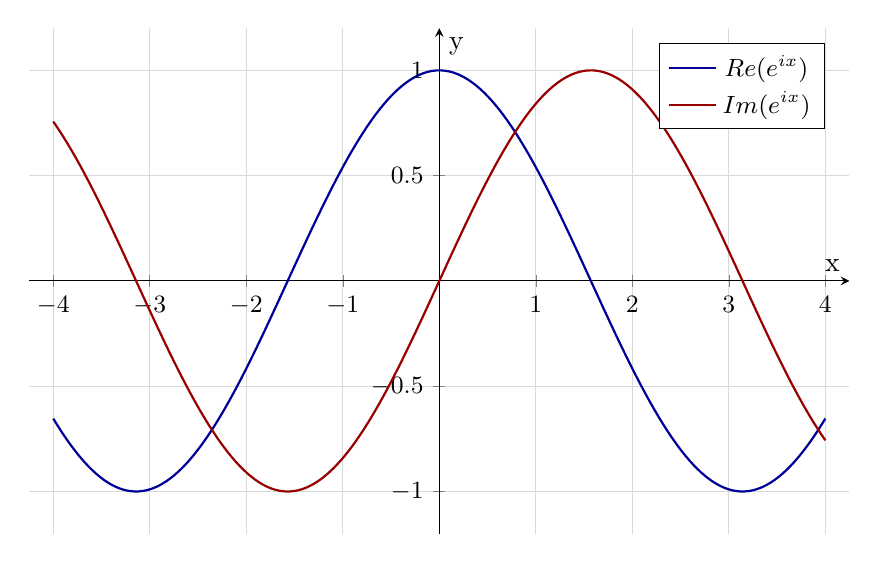
\begin{tikzpicture}
  \begin{axis}[
      xlabel={x},
      ylabel={y},
      xmin=-4.25, xmax=4.25,
      ymin=-1.2, ymax=1.2,
      grid=major,
      grid style={gray!30},
      axis lines=middle,
      width=12cm,
      height=8cm,
      xticklabel style={font=\small},
      yticklabel style={font=\small},
      legend pos=north east,
      legend style={font=\small}
    ]

    \addplot[
      domain=-4:4,
      samples=200,
      thick,
      blue!60!black
    ] {cos(deg(x))};
    \addlegendentry{$\operatorname{Re}(e^{ix})$}

    \addplot[
      domain=-4:4,
      samples=200,
      thick,
      red!60!black
    ] {sin(deg(x))};
    \addlegendentry{$\operatorname{Im}(e^{ix})$}

  \end{axis}
\end{tikzpicture}
